\documentclass[11pt,largemargins]{homework}

\newcommand{\hwname}{Dwijen Chawra}
\newcommand{\hwemail}{dchawra}
\newcommand{\hwtype}{Homework}
\newcommand{\hwnum}{3}
\newcommand{\hwclass}{CS 251}
\newcommand{\hwlecture}{}
\newcommand{\hwsection}{}

\makeatletter
\renewcommand*\env@matrix[1][\arraystretch]{%
  \edef\arraystretch{#1}%
  \hskip -\arraycolsep
  \let\@ifnextchar\new@ifnextchar
  \array{*\c@MaxMatrixCols c}}
\makeatother


\begin{document}
\maketitle

% question 0 - resources and collaborators statement
\newpage
\setcounter{questionCounter}{-1}
\question
\textbf{Problem 1:} 

Resources used: None

Collaborators: None

\textbf{Problem 2:} 

Resources used: None

Collaborators: None

\textbf{Problem 3:} 

Resources used: None

Collaborators: None

\textbf{Problem 4:} 

Resources used: None

Collaborators: None

\textbf{Problem 5:} 

Resources used: None

Collaborators: None

% Question 1
\newpage
\question

\begin{alphaparts}
  \questionpart

  Simplifying the original functions to their Big O notation:
  \begin{enumerate}[label=(\roman*)]
    \item $\log(2^{4n}) = 4n = O(n)$
    \item $log^2 4n^2 = (2 + 2 log n)^2 = O(log^2 n)$
    \item $2^{10 \log n} = n^{10} = O(n^{10})$
    \item $\log_{10}(n^{12}) = 12 \log_10 n = O(log_{10} n)$
    \item $4^{\log_2 n^2} = n^4 = O(n^4)$
    \item $4^n = O(4^n)$
    \item $\sqrt{8n} = O(\sqrt{n})$
    \item ${n}\choose{2} = \frac{n(n-1)}{2} = O(n^2)$
    \item $n^2 / \log n = O(n^2 / \log n)$
    \item $4^{2n} = O(16^{n})$
    \item $n^2 + 64n^{1.89} = O(n^2)$
  \end{enumerate}

  The functions ordered are as follows:
  \begin{enumerate}[label=(\roman*)]
    \item $\log_{10}(n^{12})$
    \item $log^2 4n^2$
    \item $\sqrt{8n}$
    \item $\log(2^{4n})$
    \item $n^2 / \log n$
    \item ${n}\choose{2}$ and $n^2 + 64n^{1.89}$
    \item $4^{\log n^2}$
    \item $2^{10 \log n}$
    \item $4^n$
    \item $4^{2n}$
  \end{enumerate}

  \newpage
  \questionpart

  \textbf{For i:} $f(n) = (\log 4n^2)^2$ vs. $g(n) = \log_{10} n^{12}$

  f(n) simplifies to $(\log 4 + log n^2)^2 = (2 + 2 \log n)^2 + 4 log n^2 + 8 log n + 4$
  % need to convert g to base 2
  g(n) simplifies to $\frac{12 \log n}{\log 10}$

  By raising the lower terms to the highest power for f(n) we get

  $f(n) = 16 \log^2 n$ vs. $g(n) = \frac{12 \log n}{\log 10}$

  Using C = 1, and k = 1, we get $16 \log^2 n \leq \frac{12 \log n}{\log 10}$ for all $n \geq 1$.

  This example is invalid, and as n approaches infinity, g(n) is never greater than f(n). 
  The fraction term in g(n) approaches 0 as n approaches infinity.
  Therefore g(n) cannot be a bound for f(n).


  \textbf{For ii)}

  $f(n) = n \choose 2$ vs. $g(n) = n^2 / log_2 n$

  Using C = 1, and k = 8, we get $\frac{n(n-1)}{2} \leq \frac{n^2}{log_2 n}$ for all $n \geq 8$.

  If we compare the behavior at infinity, the log term in g causes the function to approach 0, 
  which means that g(n) is never greater than f(n) for all $n \geq 8$.
  This means that g(n) is not a Big O bound for f(n).




  



  \textbf{For iii)}

  $f(n) = 4^n$ vs. $g(n) = 4^{2n}$

  Using C = 1, and k = 1, we get $4^n \leq 4^{2n}$ for all $n \geq 1$.

  Therefore, $f(n) = O(g(n))$.

\end{alphaparts}




% Question 2 --------------------------------------------------------------
\newpage
\question

\begin{alphaparts}
  \questionpart
  \begin{align}
    \sum_{i=1}^{n^2} \sum_{j=1}^{i} \sum_{k=1}^{\ceil*{n / 8}} 1 \\
    &= \sum_{i=1}^{n^2} \sum_{j=1}^{i} \ceil*{n / 8} \\
    &= \sum_{i=1}^{n^2} \ceil*{n / 8} \sum_{j=1}^{i} 1 \\
    &= \sum_{i=1}^{n^2} \ceil*{n / 8} i \\
    \text{Let $n^2 = k$} \\
    &= \sum_{i=1}^{k} \ceil*{n / 8} i \\
    &= \ceil*{n / 8} \sum_{i=1}^{k} i \\
    &= \ceil*{n / 8} \frac{k(k+1)}{2} \\
    &= \ceil*{n / 8} \frac{n^2(n^2+1)}{2} \\
    &= \frac{n^2(n^2+1)}{2} \ceil*{n / 8} \\
    &= \frac{n^4 + n^2}{2} \ceil*{n / 8}
  \end{align}

  \newpage
  \questionpart
  \begin{align}
    \sum_{i=1}^{n} \sum_{j=1}^{i} \sum_{k=j}^{n} 3 \\
    &= \sum_{i=1}^{n} \sum_{j=1}^{i} 3(n-j+1) \\
    &= \sum_{i=1}^{n} 3 \sum_{j=1}^{i} (n-j+1) \\
    &= \sum_{i=1}^{n} 3 (\sum_{j=1}^{i} n - \sum_{j=1}^{i} j + \sum_{j=1}^{i} 1) \\
    &= \sum_{i=1}^{n} 3 (ni - \frac{i(i+1)}{2} + i) \\
    &= 3 \sum_{i=1}^{n} (ni - \frac{i(i+1)}{2} + i) \\
    &= 3 (\sum_{i=1}^{n} ni + \sum_{i=1}^{n} i - \sum_{i=1}^{n} \frac{i(i+1)}{2}) \\
    &= 3 (n \sum_{i=1}^{n} i + \sum_{i=1}^{n} i - \frac{1}{2} \sum_{i=1}^{n} i^2 - \frac{1}{2} \sum_{i=1}^{n} i) \\
    &= 3 (\frac{n^2(n+1)}{2} + \frac{n(n+1)}{2} - \frac{n(n+1)(2n+1)}{12} - \frac{3n(n+1)}{12}) \\
    &= 3(\frac{n^{3}+n^{2}}{2}-\frac{1}{2}(\frac{2n^{3}+3n^{2}+n}{6}+\frac{n^{2}+n}{2})+\frac{n^{2}+n}{2}) \\
    &= 3(\frac{2n^{3}+2n^{2}}{4}-\frac{2n^{3}+3n^{2}+n}{12}-\frac{n^{2}+n}{4}+\frac{2n^{2}+2n}{4}) \\
    &= 3(\frac{2n^{3}+4n^{2}+2n}{4}-\frac{2n^{3}+3n^{2}+n}{12}-\frac{n^{2}+n}{4}) \\
    &= \frac{6n^{3}+9n^{2}+3n}{4}-\frac{2n^{3}+3n^{2}+n}{4} \\
    &= \frac{2n^{3}+3n^{2}+n}{2}
  \end{align}

  \newpage
  \questionpart

  Adding 1 because of Edstem, and assuming n is a power of 4 also according to Ed.

  % Using recurrence:

  % \begin{align}
  %   T(n) &= T(n/4) + T(n/4) \\
  %   &= 2T(n/4) \\
  %   &= 2(2T(n/16)) \\
  % \end{align}
  
  \begin{align}
    \sum_{i=1}^{\log_4 n^2 + 1} 1 \\
    &= \sum_{i=1}^{\log_4 n^2} 1 + 1 \\
    &= \log_4 n^2 + 1 \\
    &= 2 \log_4 n + 1
  \end{align}

  \questionpart

  \begin{align}
    \sum_{i=1}^{n} \sum_{j=1}^{\floor*{log n} + 1} 1 \\
    &= \sum_{i=1}^{n} \floor*{log n} + 1 \\
    &= n \floor*{log n} + 1
  \end{align}

\end{alphaparts}

% Question 3
\newpage
\hspace{-5em}
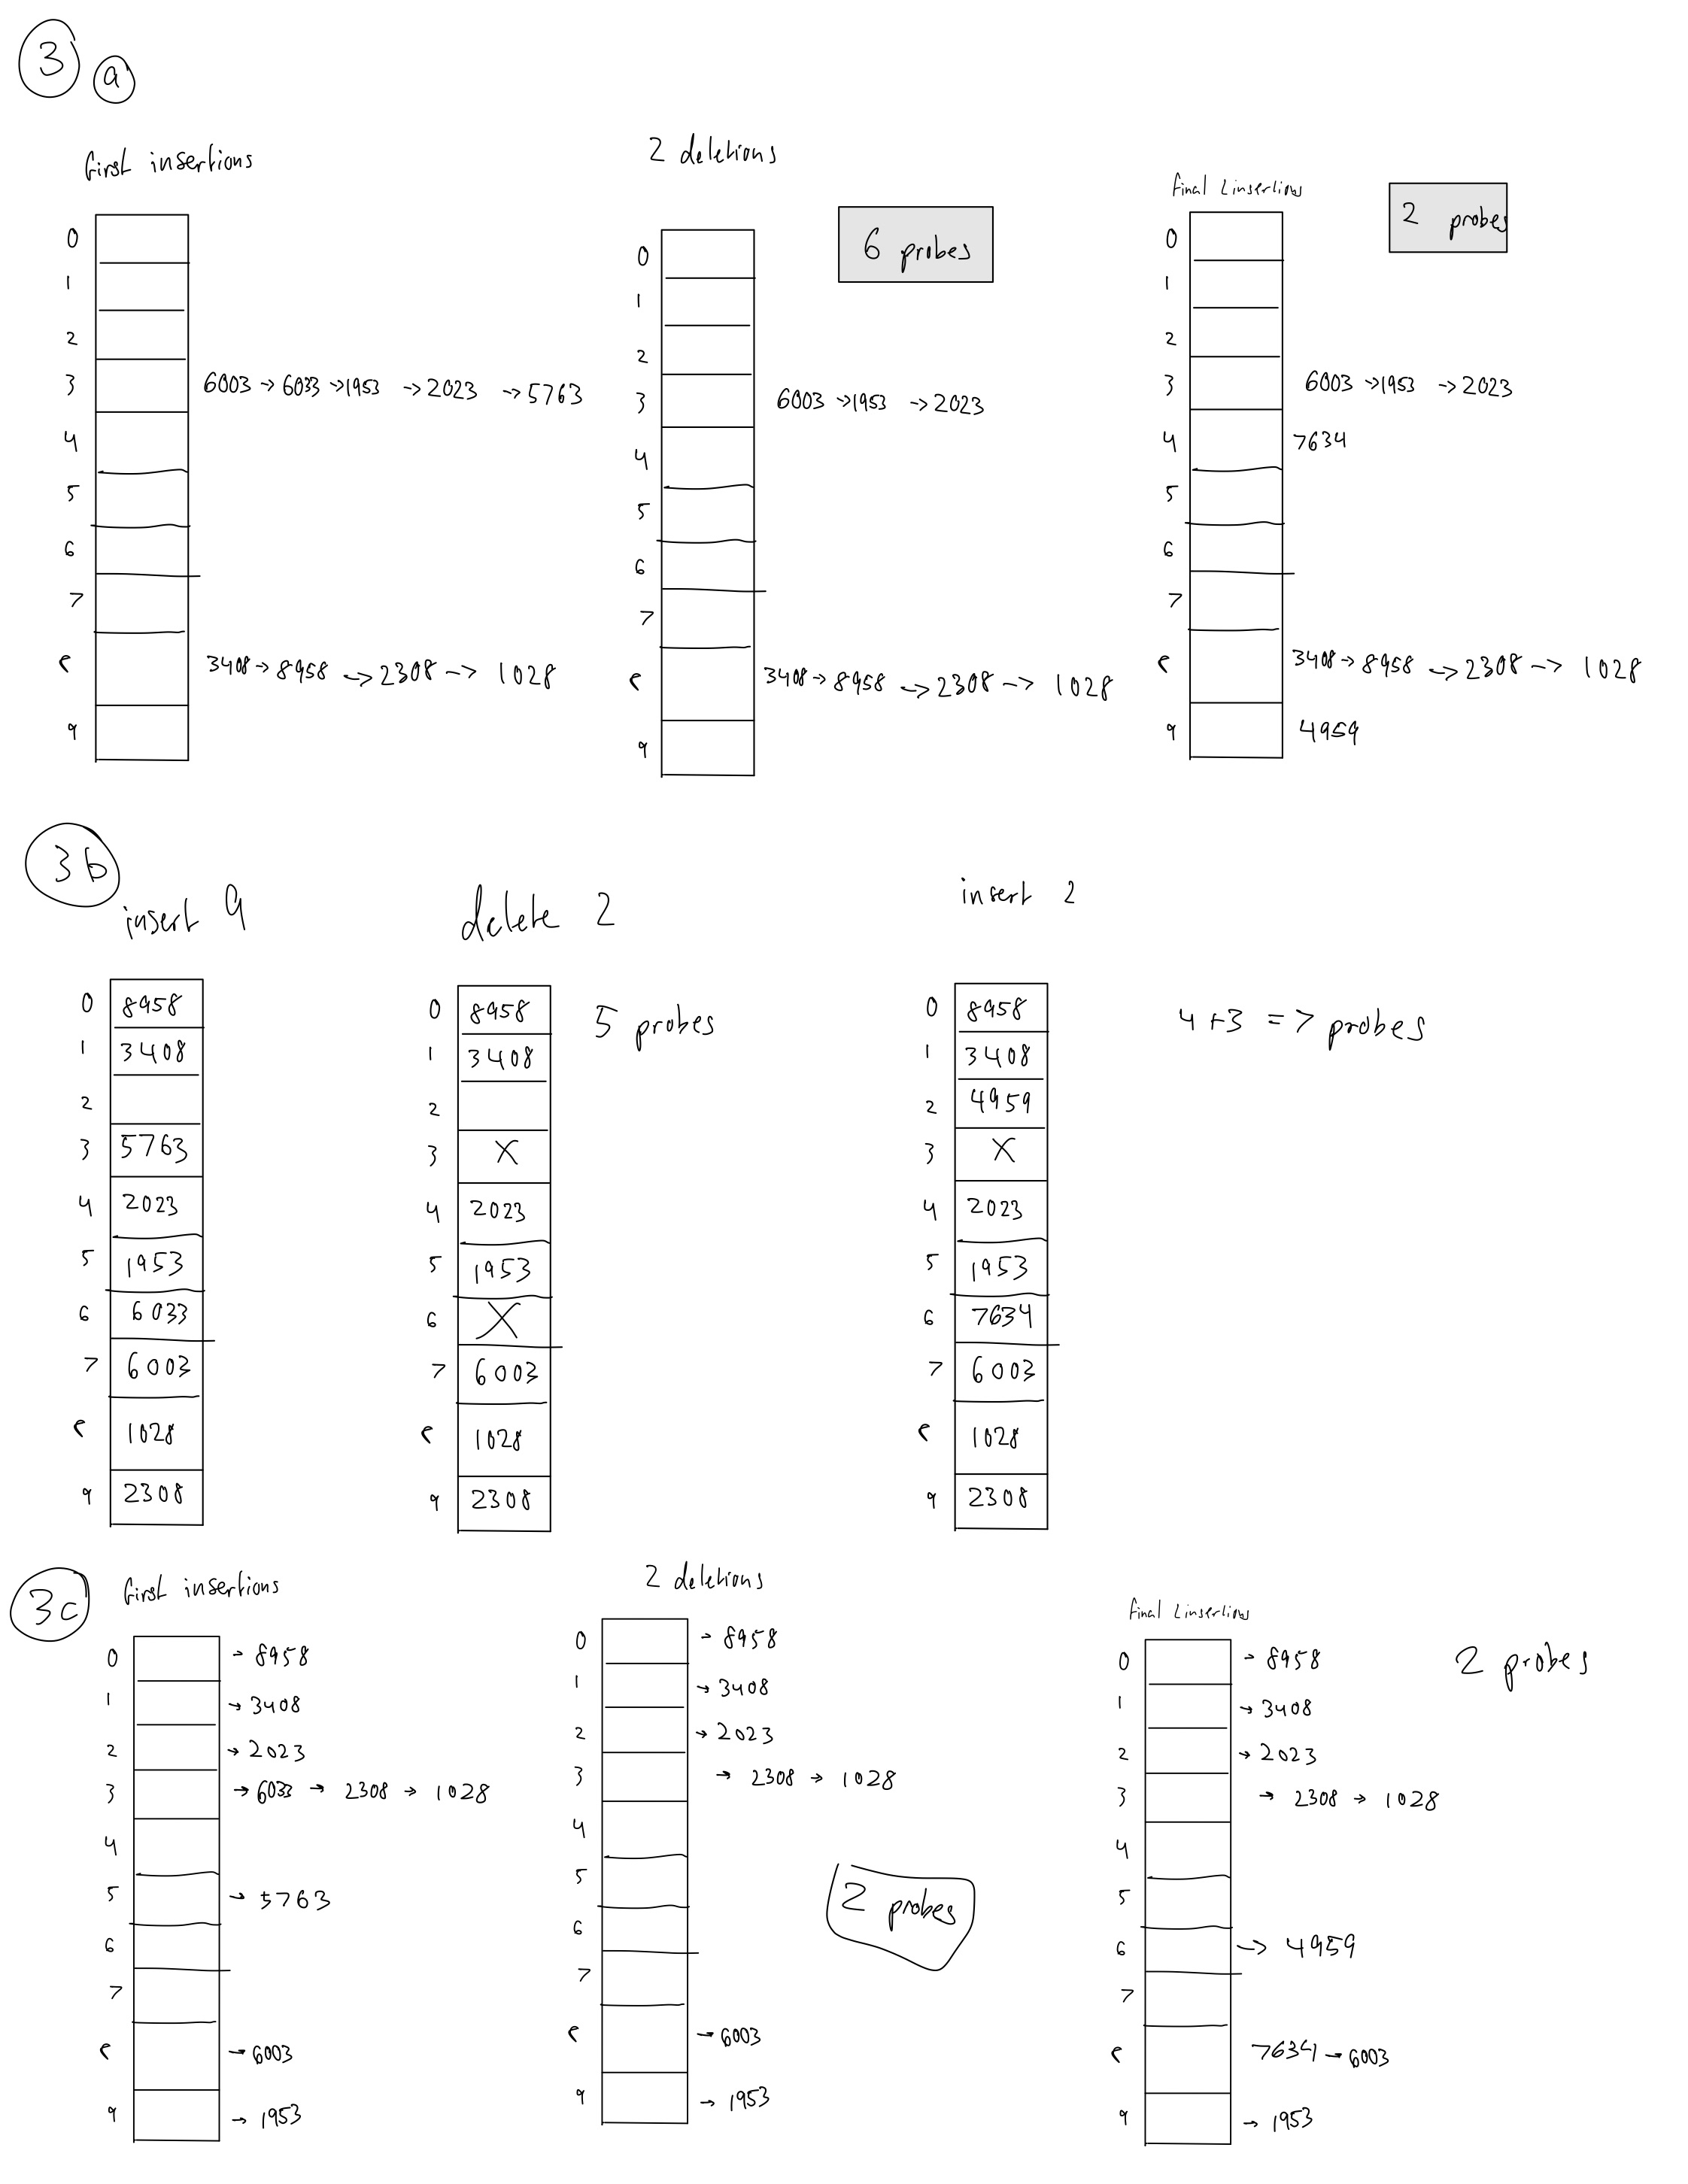
\includegraphics[width=1.3\textwidth]{pictures/hw3/q3abc.jpg}
\newpage
\hspace{-5em}
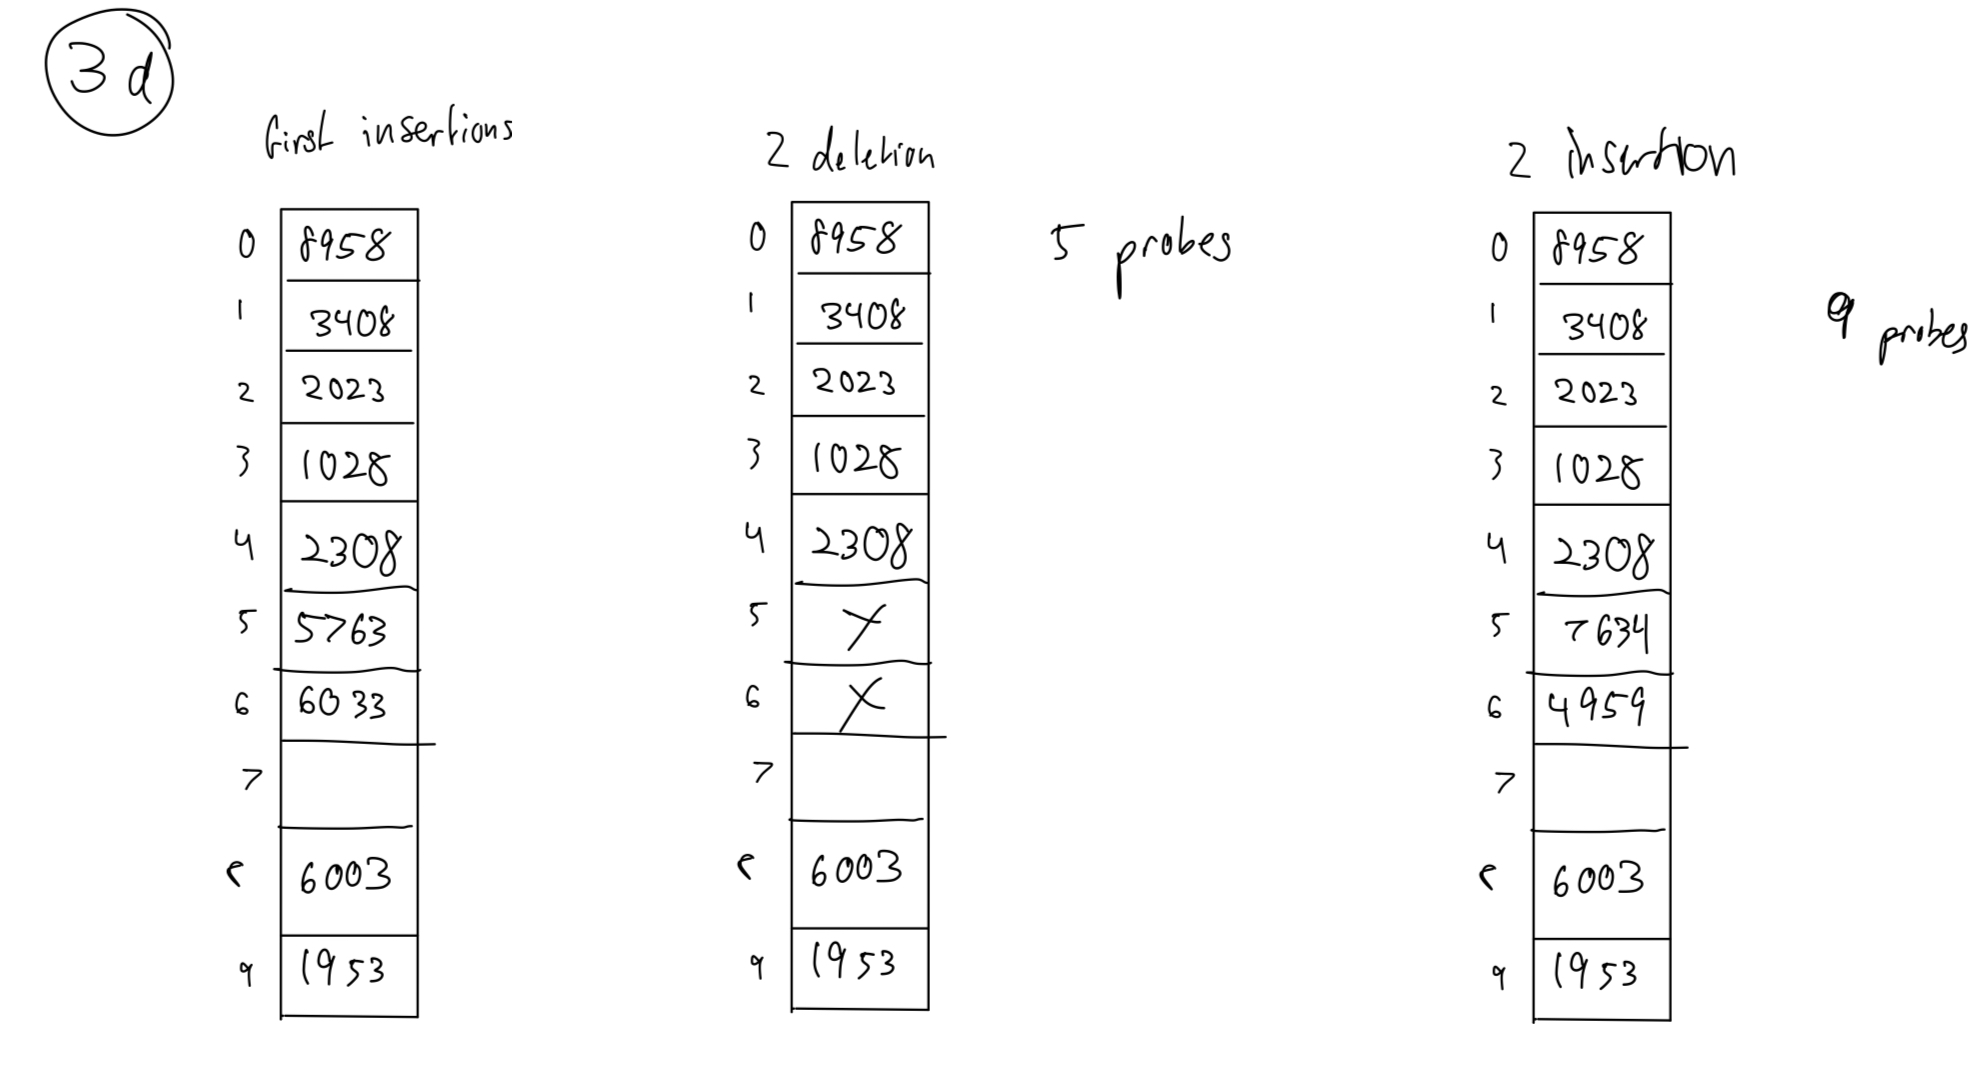
\includegraphics[width=1.3\textwidth]{pictures/hw3/q3d.jpeg}


% Question 4
\newpage
\setcounter{questionCounter}{3}
\question

\begin{alphaparts}
  \questionpart
  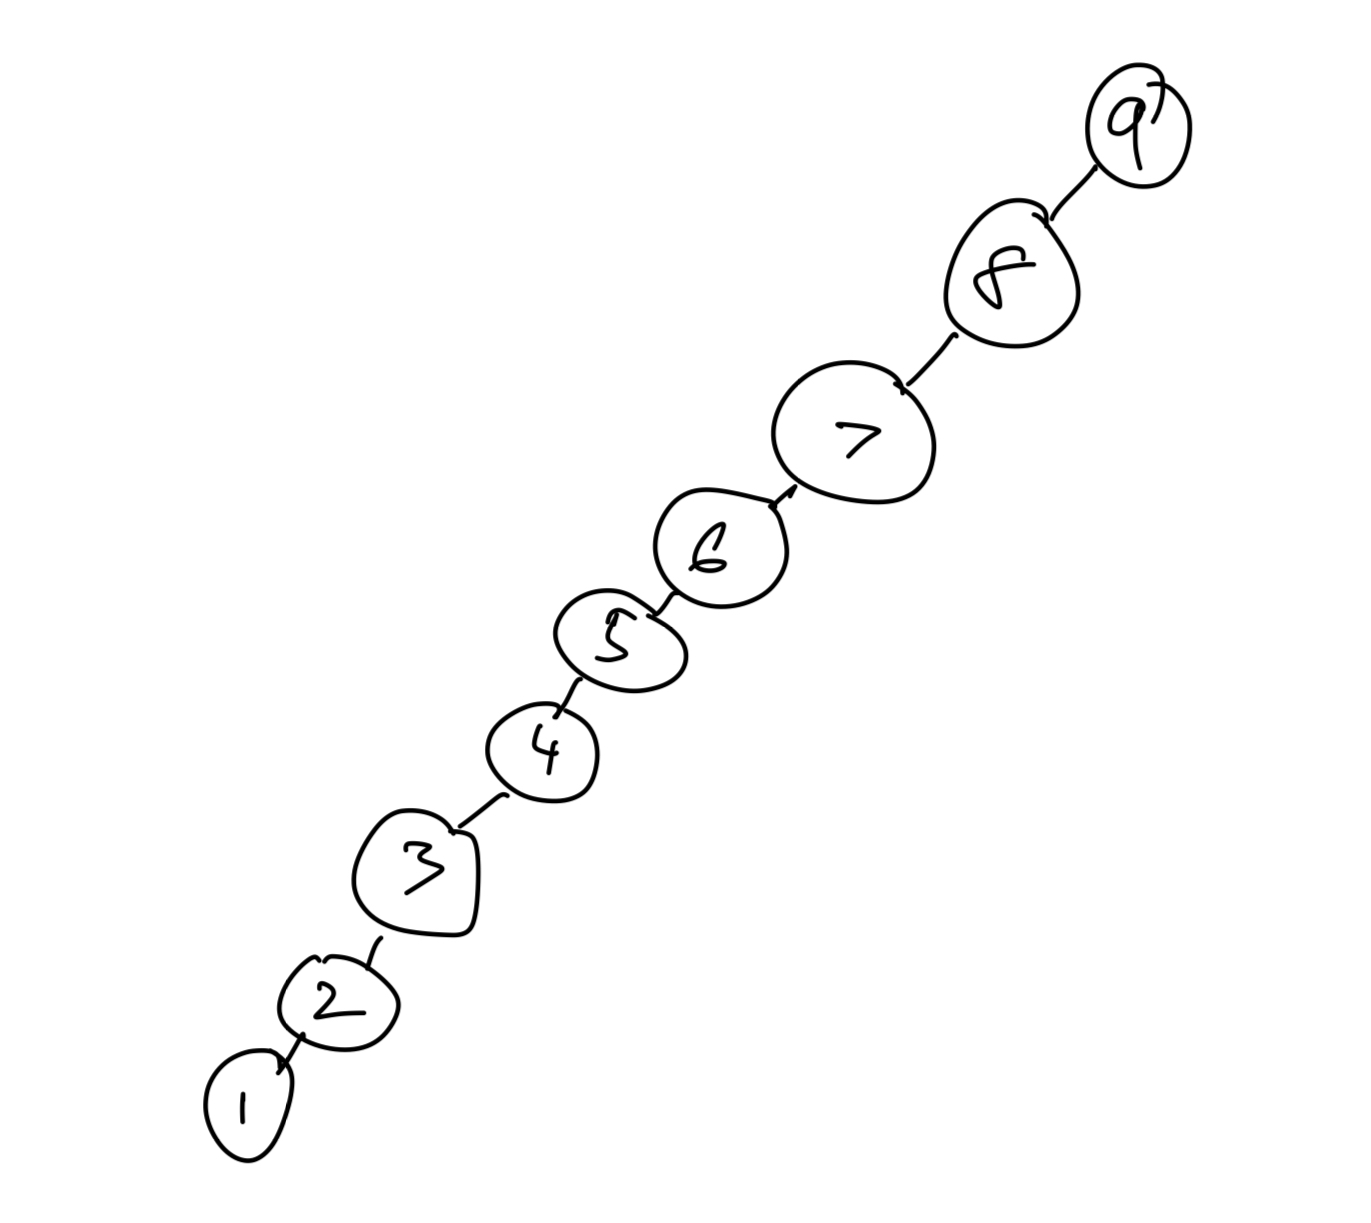
\includegraphics[width=0.5\textwidth]{pictures/hw3/q4a.jpeg}

  Assuming n, n-1, n-2, ... 1 are inserted into a BST, the runtime of this would be O($\sum_{i=1}^{n} 1$).
  This is because the first element inserted would be an O(1) operation, then O(2), and so on until O(n).
  The resulting runtime is O($\sum_{i=1}^{n} 1$) = O($\frac{n(n+1)}{2}$) = O($n^2$).

  % prove big theta for this

  To get big theta we need to prove that the runtime is also $\Omega(n^2)$.
  $\Omega$ for this would be the same, because there is no better way to insert the elements in descending order; we have to traverse the left child every time.
  
  f(n) = O($n^2$) and g(n) = $n^2$

  When C = 1, and k = 1, $n^2 \leq C \cdot n^2$

  
  Therefore, the runtime is $\Theta(n^2)$.

  \questionpart
  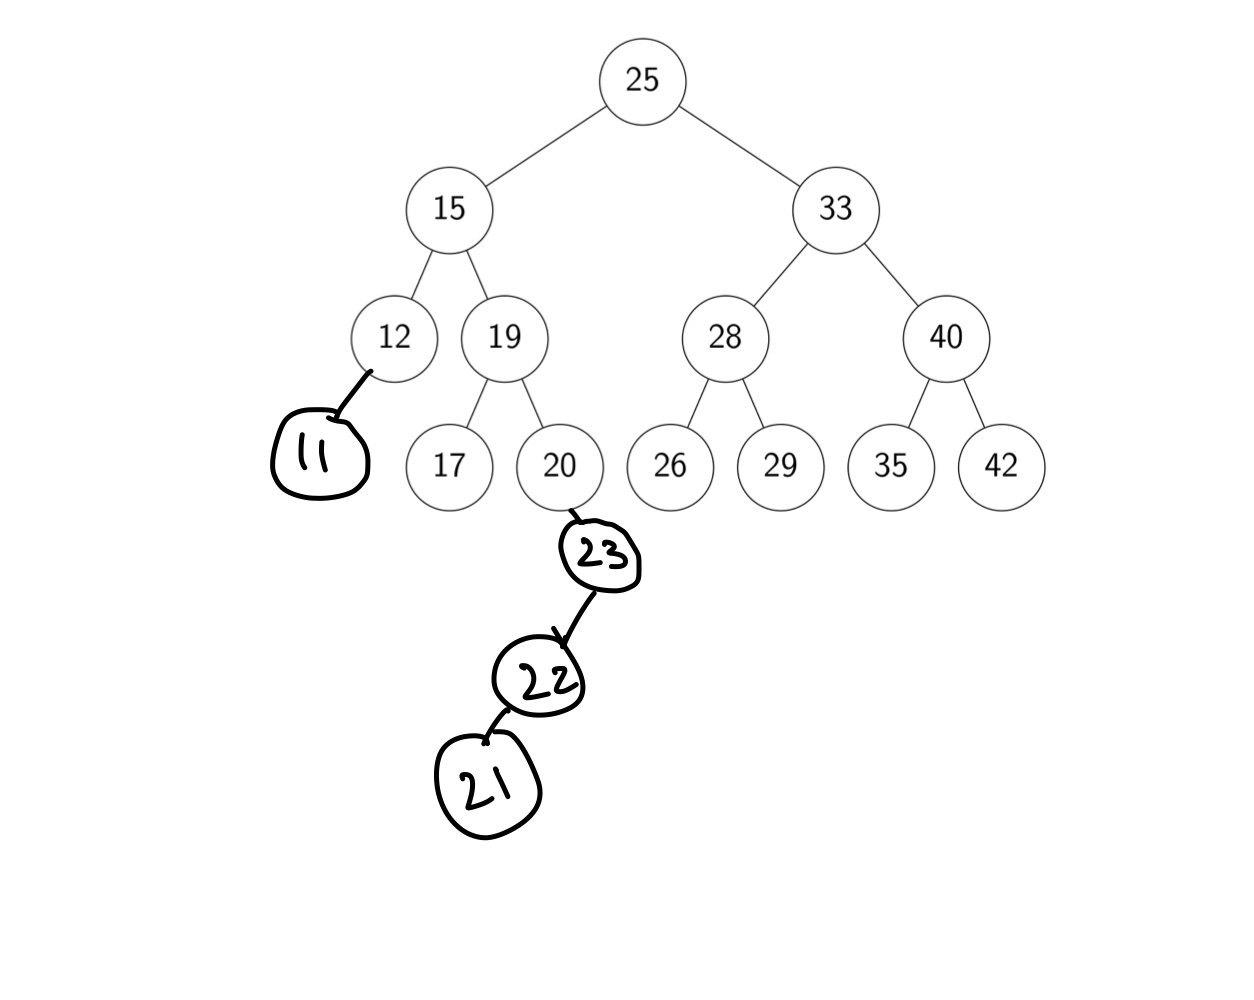
\includegraphics[width=0.7\textwidth]{pictures/hw3/q4b.jpeg}

  \questionpart
  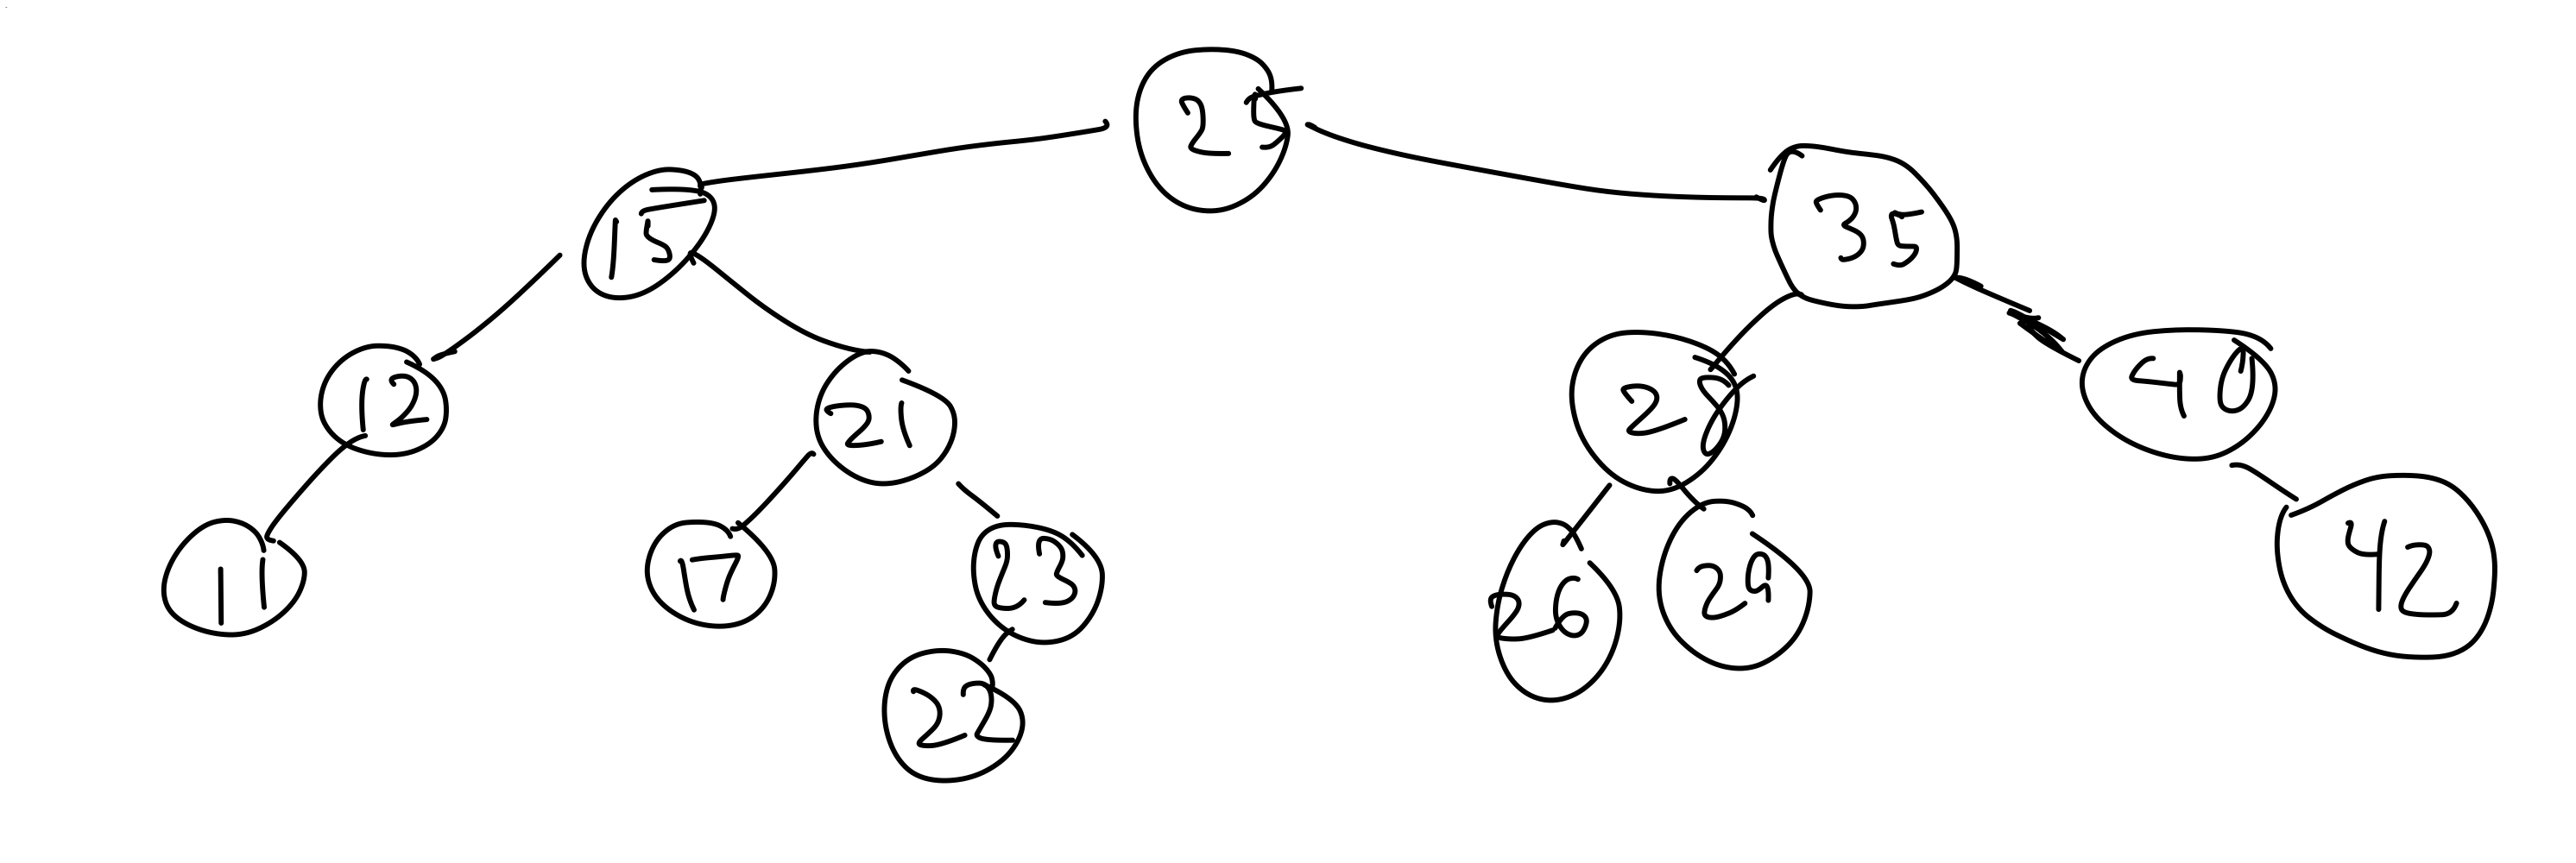
\includegraphics[width=0.9\textwidth]{pictures/hw3/q4c.jpeg}

  del 19: 19 had 2 children, so we replace 19 with min(right), which is 20.
  20 has one child, so we replace 20 with 21. 21 has no children, so we delete it.

  del 33: 33 had 2 children, so we replace 33 with min(right), which is 35.
  35 has no children, so we delete it.

  del 20: 20 has one child, so we take the min of the right subtree, which is 21, then delete 21.
  \questionpart
  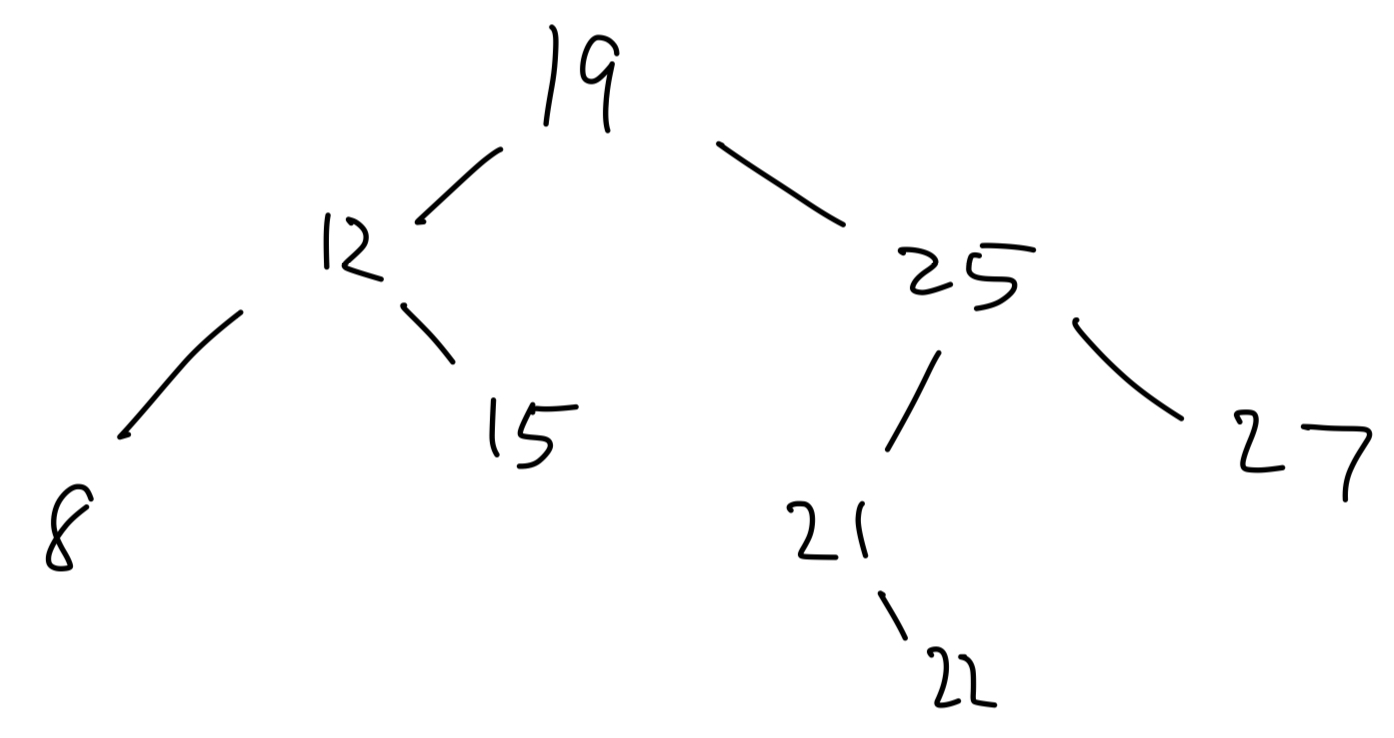
\includegraphics[width=0.9\textwidth]{pictures/hw3/q4d.jpeg}


\end{alphaparts}


\end{document}
